% Original vector graph reconstruction, source Fig.60.1, PDF250/printed238.
% Arrow labels give fermion flow; the exchanged photon momentum points upward.
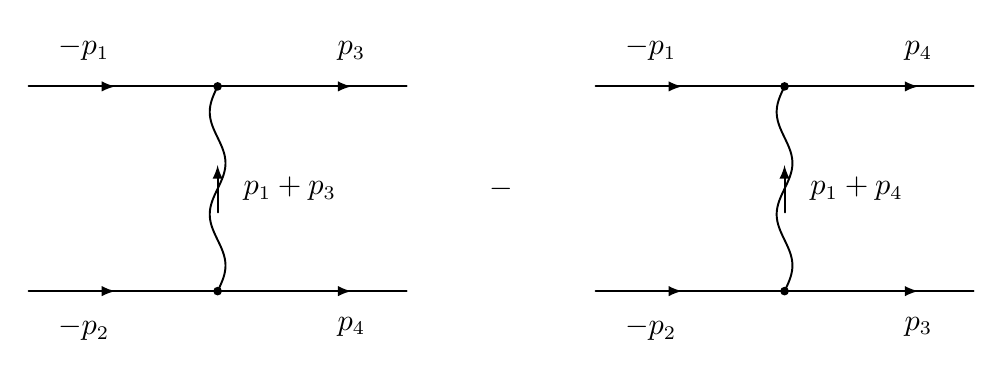
\begin{tikzpicture}[x=1mm,y=1mm,line width=.7pt,>=latex,
 line cap=round,line join=round,font=\fontsize{10.5}{12}\selectfont]
 \foreach \offset in {0,72}{
  \begin{scope}[shift={(\offset,0)}]
   \foreach \height in {13,-13}{
    \draw (0,\height)--(48,\height);
    \draw[->] (5,\height)--(11,\height);
    \draw[->] (35,\height)--(41,\height);
    \fill (24,\height) circle[radius=.55mm];
   }
   \draw[domain=0:26,samples=101,smooth,variable=\u]
    plot ({24+1.0*sin((\u/26)*720)},{-13+\u});
   \draw[->] (24,-3)--(24,3);
   \node[above] at (7,15) {$-p_1$};
   \node[below] at (7,-15) {$-p_2$};
  \end{scope}
 }
 \node[above] at (41,15) {$p_3$};
 \node[below] at (41,-15) {$p_4$};
 \node[right] at (26,0) {$p_1+p_3$};
 \node at (60,0) {$-$};
 \node[above] at (113,15) {$p_4$};
 \node[below] at (113,-15) {$p_3$};
 \node[right] at (98,0) {$p_1+p_4$};
\end{tikzpicture}
